\documentclass[12pt,a4paper]{article}

\renewcommand{\baselinestretch}{1.3}

\usepackage[left=1.5cm,right=1.5cm,top=2cm,bottom=2.5cm]{geometry}
\usepackage{graphicx} 
\graphicspath{{Pics/}}
\DeclareGraphicsExtensions{.pdf, .png, .tif, .eps, .tiff, .psd, .jpg}
\usepackage{setspace}
\usepackage{indentfirst}
\usepackage{array}
\usepackage[T2A]{fontenc}
\usepackage[utf8]{inputenc}
\usepackage[russian]{babel}
\usepackage{amsmath}
\usepackage{amssymb}
\usepackage{graphicx}
\usepackage{tikz}
\usepackage{comment}
\usepackage{enumerate}
\usepackage{wrapfig}
\usepackage{verbatim}
\usepackage{amsmath}
\pagestyle{plain}

\usepackage{mathtools}
\DeclarePairedDelimiter{\ceil}{\lceil}{\rceil}

\RequirePackage{caption}
\DeclareCaptionLabelSeparator{dot}{ . }
\captionsetup{justification=centering, labelsep=dot}


\begin{document}

\begin{center}
	\large \textbf{Алгебра} \\ 1 курс, 2 модуль\\ Фейгин Евгений Борисович
\end{center}
	
	\tableofcontents
	\newpage 
	
\section{Группы (29.10.19)}

\textbf{Определение.} Группа --- это множество G с одной операцией, удовлетворяющей следующим свойствам: 

(1) (ab)c = a(bc);

(2) $\exists e \in G: \forall a \in G ea = ae = a;$

(3) $\forall a \in G \; \exists a^{-1} \in G: aa^{-1} = a^{-1}a = e.$

\textbf{Примеры:} $\; \bullet \; \mathbb{R}_{+}$ --- вещественные числа по сложению; 

$\quad \quad \quad \quad \quad \quad \bullet \; \mathbb{R}_{+}^{+}$ --- вещественные положительные числа по сложению; 

$\quad \quad \quad \quad \quad \quad\bullet \; \mathbb{Z}/_{n\mathbb{Z}}$ --- вычеты по модулю n по сложению;

$\quad \quad \quad \quad \quad \quad\bullet \; \mathbb{F}^{*} = \mathbb{F} \backslash 0$ --- группа обратных элементов поля. 

\textbf{Определение.} Абелева (коммутативная) группа: $\forall a, b \in G \; ab = ba.$

Пусть X --- множество. Обозначим через S(x) множество всевозможных взаимно-однозначных отображений $X \to X$ с операцией композиции. 

\textbf{Пример.} X --- конечное множество из n элементов. S(X) обозначим через $S_n$, n = |X|. Например, X может быть $\{1, ..., n\}.$ 

\textbf{Пример.} Пусть V --- векторное пространство над полем $\mathbb{F}$. Рассмотрим все преобразования V вида $t_a: V \to V, \; t_{a}(V) = V + a, a \in V$. Тогда $t_{a}t_{b}: V \to V, \; t_{a}t_{b}(V) = V + a + b = t_{a} + b$. Таким образом, V образует группу по сложению. 

\textbf{Определение.} Подмножество $H \subset G$ называется подгруппой (и также является группой), если 

(1) $e \in H$; 

(2) $a, b \in H \Rightarrow ab \in H$; 

(3) $a \in H \Rightarrow a^{-1} \in H$. 

\textbf{Определение.} Гомоморфизм групп: отображение $\varphi: G_{1} \to G_{2}$, где $G_{1}, G_{2}$ --- группы, т.ч. $\varphi(g_{1}, g_{2}) = \varphi(g_{1})\varphi(g_{2}), \; \varphi(a^{-1}) = \varphi(a)^{-1}.$

Гомоморфизм $\varphi$ называется изоморфизмом, если $\varphi$ взаимно-однозначно. Автоморфизм --- изоморфизм $\varphi: G \to G$. 

\textbf{Пример.} Группа G называется циклической, если $\exists g \in G: \forall g_{1} \in G \exists k \in \mathbb{Z}: g_{1} = g^{k}$. 

\textbf{Лемма.} Любая циклическая группа изоморфна $\mathbb{Z}/_{n\mathbb{Z}}, \; n \geq 1$ или $\mathbb{Z}$ относительно сложения. 

\textbf{Доказательство.} Если существует минимальное n т.ч. $g^{n} = e$ (g --- образующая циклической группы), то $G \mapsto \mathbb{Z}/_{n\mathbb{Z}}$ строится по формуле $g^{k} \mapsto [k], e \mapsto [0]$. Если существует k т.ч. $g^{k} = e$, то $G = {g^{k}, \; k \in \mathbb{Z}}, \; g^{k} \neq g^{l}$, если $k \neq l$. Тогда G изоморфно $\mathbb{Z}, \; g^{k} \mapsto k$.

\textbf{Определение.} Множество элементов $S = \{g_{1}, g_{2}, ..., g_{n}\}$ называется образующими группы $G \; (g_{i} \in G)$, если минимальная подгруппа $H \subset G$, содержащая все $g_i$, совпадает с G. Другими словами, $\forall g \in G, g = g_{i_1}^{\epsilon_{1}} g_{i_2}^{\epsilon_{2}}...g_{i_m}^{\epsilon_m}$, где $\epsilon_k = \pm 1, \; i = 1, ..., k, \; m \geq 0$. 

\textbf{Пример.} $g_{1}g_{1}g_{1}g_{1}$, то есть в записи выше $g_{i_k}$ необязательно различны. 

\textbf{Замечание.} Если k = 1, то G циклическая. 

\textbf{Пример.} Группа $S_3$ не является циклической, но порождена двумя элементами. S = {(12), (23)}. 

\textbf{Лирическое отступление.} $S_{n} = S(\{1, ..., n\}), (ij) \in S_{n}, (ij)$ --- транспозиция. $i_1 \mapsto i_2, ..., i_k \mapsto i_1, j \mapsto j, j \notin \{i_1, ..., i_k\}$. 

\textbf{Предложение.} Группа $S_n$ имеет несколько наборов образующих: $(1 2), (2 3), ..., ((n - 1) k); (1 2), (1 3), ..., (1 n)$. 

\textbf{Пример.} Свободная группа с двумя образующими $g_1, g_2$ --- группа, состоящая из элементов $g_{i_1}^{\epsilon_{1}} g_{i_2}^{\epsilon_{2}}...g_{i_m}^{\epsilon_m}$, i = 1, 2, $\epsilon = \pm 1, m \geq 0.$ Все такие элементы разные с точностью до сокращения $g_{1}g_{1}^{-1} = e, g_{2}g_{2}^{-1} = e, g_{1}g_{2} \neq g_{2}g_{1}$. 

\textbf{Пример.} $S_3: g_1 = (12), g_2 = (23), g_{1}g_{2}g_{1} = g_{2}g_{1}g_{2}$ --- соотношение кос, $g_{1}^2 = e$. 

\subsection{Ортогональные преобразования плоскости}

\textbf{Определение.} Группа О(2) --- группа линейных преобразований $\mathbb{R^2}$, сохраняющая расстояние. Любое линейное преобразование $\mathbb{R}^2$ задается матрицей $\begin{pmatrix}
	a&b\\
	c&d
\end{pmatrix}$ т.ч. $\begin{pmatrix}
a&b\\
c&d
\end{pmatrix}$ $\begin{pmatrix}
x\\
y
\end{pmatrix}$ = $\begin{pmatrix}
ax + by\\
cx + dy
\end{pmatrix}$

$\begin{pmatrix}
a&b\\
c&d
\end{pmatrix} \in O(2) \Leftrightarrow (ax + by)^2 + (cx + dy)^2 = x^2 + y^2.$

$a^2 + c^2 = 1, b^2 + d^2 = 1, ab + cd = 0 \Rightarrow a = \cos \alpha, c = \sin \alpha \Rightarrow \left[ 
\begin{gathered} 
b = \sin \alpha, d = -\cos \alpha; \\ 
b = -\sin \alpha, d = \cos \alpha. \\ 
\end{gathered} 
\right.$

$\begin{pmatrix}
\cos \alpha & \sin \alpha\\
\sin \alpha & -\cos \alpha
\end{pmatrix} \rightarrow \det = -1$, $\begin{pmatrix}
\cos \alpha & -\sin \alpha\\
\sin \alpha & \cos \alpha
\end{pmatrix} \rightarrow \det = 1$

\textbf{Замечание.} Иногда O(2) обозначается $I_{SO}(\mathbb{R}^2)$. 

\textbf{Замечание.} Имеется O(3), O(4), $...$. 

\textbf{Определение.} Пусть $x \subset \mathbb{R}^2$. Тогда $I_{SO}(x) = \{g \in O(2): gx = x\}.$ 

\textbf{Утверждение.} $I_{SO}(x)$ --- подгруппа в O(2). 

\textbf{Доказательство.} $l \in I_{SO}(x) \; (l = \pm d), g_{1}, g_{2} \in I_{SO}(x) \Leftrightarrow g_{1}g_{2}, g_{1}^{-1} \in I_{SO}(x)$. 

\textbf{Пример.} X --- правильный n-угольник. $I_{SO}(x) = D_{n}$ --- группа диэдра (группа (конечная) симметрии правильного многоульника, включающая вращения и осевые симметрии, --- мое примечание). 

\subsection{Смежные классы}

\textbf{Обозначается} $g \in G$, ord g = min\{k: $g^k = 1\} \in \mathbb{Z}_{\geq 0} \cup {\infty}.$

Пусть H --- подгруппа в G. Тогда любое множество вида gH = {gh: $h \in H$} называется \textbf{правым смежным классом.} Hg = {hg: $h \in H$} --- \textbf{левый смежный класс.} 

\textbf{Свойства:} $ \bullet \; |gH| = |Hg| = |H|,$ так как $gh_{1} = gh_{2} \Rightarrow h_{1} = h_{2};$

$\quad \quad \quad \quad \quad \quad \bullet$ H является как левым, так и правым смежным классом;

$\quad \quad \quad \quad \quad \quad\bullet$ 2 левых/правых смежных класса либо совпадают, либо не пересекаются. 

\textbf{Доказательство.} $g_{1}H = g_{2}H \neq \emptyset \Leftrightarrow \exists h_{1}, h_{2}: g_{1}h_{1} = g_{2}h_{2} \Leftrightarrow g_{1}h_{1}h_{2}^{-1} = g_{2} \Leftrightarrow g_{1}H = g_{2}H.$ 

\begin{wrapfigure}{R}{0.3\textwidth}
	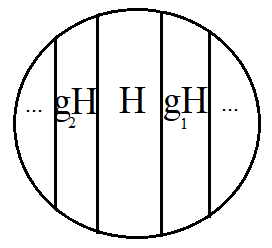
\includegraphics[width=0.8\linewidth]{Pic1}
\end{wrapfigure}

\textbf{Следствие --- теорема Лагранжа.} $|H| | |G| \Leftrightarrow |G| \; \vdots \; |H|$ --- порядок группы делится на порядок подгруппы. 

\textbf{Следствие.} Пусть H = <g> --- подгруппа, порожденная $g \in G$. Тогда если $|G| < \infty, |H| < \infty$, то $|G| \; \vdots$ ord g. 

\textbf{Следствие.} Любые две группы из $p \in \mathbb{P}$ элементов изоморфны. 

\textbf{Доказательство.} $\forall g \in G$ ord g = $\begin{cases}
1 \rightarrow \; $ord g = 1$ \Leftrightarrow g = l,\\
p \rightarrow \forall g \neq l \; $ord g = p$ \; \Rightarrow G$ --- циклическая.$ 
\end{cases}$

\textbf{Следствие.} Количество правых (левых) смежных классов равно $|G|_{/|H|}.$

\textbf{Определение.} Подгруппа $H \subset G$ называется \textbf{нормальной}, если множества правых и левых смежных классов совпадают, то есть $\forall g \in G gH = Hg$. 

\textbf{Замечание.} Определение равносильно $gHg^{-1} = H \; \forall g \in G.$

\textbf{Замечание.} $gH = Hg \Leftrightarrow h_{1} \in H \; \exists h_{2} \in H$ т.ч. $gh_{1} = h_{2}g$. 

\textbf{Определение.} $\varphi: G_{1} \to G_{2}$ --- гомоморфизм групп ker$\varphi = \{g \in G_{1} =: \varphi(g) = e\},$ Im$\varphi = \{g_{2} \in G_{2}: \exists g_{1} \in G_{1}: \varphi(g_{1}) = g_{2}\}.$ 

\textbf{Лемма.} ker$\varphi$ --- нормальная подгруппа в $G_{1}$. 

\textbf{Доказательство.} $\bullet \; \ker \varphi$ --- подгруппа, так как $e \in \ker \varphi (\varphi(e) = e); g_{1}g' \in \ker \varphi \Leftrightarrow \varphi(gg') = \varphi(g)\varphi(g') = ee = e.$

$\bullet \;$ Пусть $x \in G_{1}, \; g \in \ker \varphi.$ Тогда $\varphi(xgx^{-1}) = \varphi(x)\varphi(g)\varphi(x^{1}) = \varphi(x)\varphi(x)^{-1} = e.$ Т.о., $xgx^{-1} \in \ker \varphi,$ то есть $\ker \varphi$ нормально.

\begin{wrapfigure}{R}{0.3\textwidth}
	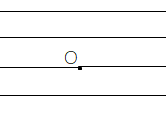
\includegraphics[width = 5cm]{5_11_1.png}
\end{wrapfigure}

\textbf{Замечание.} Пусть H --- нормальная подгруппа, $g \in G.$ $gHg^{-1} \subset H,$ то есть элемент $g \in G$ задает отображение $adg: H \to H, (adg)(h) = ghg^{-1}.$ Что означает, что $(adg)h_{1} = (adg)h_{2} \Leftrightarrow gh_{1}g^{-1} \Leftrightarrow h_{1} = h_{2}.$ То есть если H конечна, то достаточно требовать, что $gHg^{-1} \subset H.$ 

\textbf{Примеры.} $\bullet \; G = \mathbb{Z}, \; H = h\mathbb{Z}$ (относительно сложения). Смежные классы: $\{a + kn, \; k \in \mathbb{Z}\} = [a].$

\textbf{Замечание.} Если G --- это коммутативная группа, то любая ее подгруппа нормальна $(gHg^{1} = gg^{-1}H = H).$

$\bullet \; G = (\mathbb{C}, +), H = (\mathbb{R}, +) = \{z: Im z = 0\}$, смежные классы: (картинка справа)

\begin{wrapfigure}{R}{0.3\textwidth}
	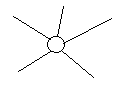
\includegraphics[width = 5cm]{5_11_2.png}
\end{wrapfigure}

$\bullet \; G = (\mathbb{C}\backslash\{0\}; \times); H = (\mathbb{R}_{> 0}, \times),$ смежные классы: (картинка справа)

\begin{wrapfigure}{R}{0.3\textwidth}
	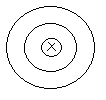
\includegraphics[width = 5cm]{5_11_3.png}
\end{wrapfigure}

$\bullet \; G = (\mathbb{C}\backslash\{0\}, \times), H = S^{1} = \{z: |z| = 1\},$ смежные классы: (картинка справа)

$\bullet \; G = S_{n}, h = S_{n - 1} = \{\sigma \in S_{n}: \; \sigma(n) = n\}.$ Хотим описать левые смежные классы. $\sigma \in S_{n}, \; H\sigma = \{g \in S_{n}: g^{-1}(n) \sigma^{-1}(n)\}.$ Пусть $g = h\sigma: g^{1}(n) = (h\sigma)^{-1}(n) = (\sigma^{-1}h^{-1})(n) = \sigma^{-1}(n).$ Пусть $g in S_{n}, g^{-1}(n) = \sigma^{-1}(n).$ Тогда мы хотим проверить, что g = hG для некоторого $h \in H,$ то есть $g\sigma^{-1} \in H \Leftrightarrow (g\sigma^{-1})(n) = n \Leftrightarrow \sigma^{-1}(n) = g^{-1}(n).$ 

Правые смежные: $\sigma H = \{\sigma h: h(n) = n\} = \{g \in S_{n}: g(n) = \sigma(n)\}.$

\textbf{Вывод.} $S_{n - 1} \subset S_{n}$ --- ненормальная подгруппа. 

\textbf{Замечание.} $\psi: \; G \to G, \; \psi(g) = g^{-1}$ --- антиавтоморфизм (умножение не переводится в умножение: $\psi(g_{1}g_{2}) = (g_{1}g_{2})^{-1} = g_{2}^{-1}g_{1}^{-1} = \psi(g_{2})\psi(g_{1}). \; H \in G, \psi(GH) = H\sigma^{-1}.$ То есть $\psi$ осуществляет биекцию между правыми и левыми смежными классами. 

$H \subset G, g_{1}H\cdot g_{2}H = g_{1}g_{2}H \; \Leftrightarrow \; [g_{1}][g_{2}] = [g_{1}g_{2}], \; [g] = gH$ --- смежный класс g.  

\textbf{Предложение.} Формула $g_{1}Hg_{2}H = g_{1}g_{2}H$ определяет корректно заданное умножение на множестве смежных классов $\Leftrightarrow$ H нормальна в G. 

\textbf{Доказательство.} Пусть группа нормальна. Хотим проверить, что если $f_{1} \in [g_{1}], f_{2} \in [g_{2}],$ то $[f_{1}f_{2}] = [g_{1}g_{2}]. \; f_{1} = g_{1}h_{1}, \; f_{2} = g_{2}h_{2} \Leftrightarrow f_{1}f_{2} = g_{1}h_{1}g_{2}h_{2} = g_{1}g_{2}(g_{2}^{-1}h_{1}g_{2} (\in H)) h_{2} = g_{1}g_{2} h$(c крышечкой),  где h (с волной) = $g_{2}^{-1}h_{1}g_{2})h_{2} \in H \Rightarrow [f_{1}f_{2}] = [g_{1}g_{2}],$ то есть умножение корректно определено. 

Тогда на множестве смежных классов [G:H] возникает структура группы: 

$e = [e] = H, [g]^{-1} = [g^{-1}], [g_{1}(g_{2}g_{3})] = [g_{1}][g_{2}g_{3}] = [g_{1}]([g_{1}][g_{2}])[g_{3}],$ где $[g_{1}(g_{2}g_{3})] = [(g_{1}g_{2})g_{3}] = [g_{1}g_{2}][g_{3}] = ([g_{1}][g_{2}])[g_{3}].$

$\tau: G \to G_{H}$ --- фактор группа, G фактор по H, $\tau(g) = [g]$ --- отображение факторизации, где  через $G_{H}$ обозначается группа, элементами которой являются смежные классы. Тогда $\tau$ --- гомоморфизм групп, то есть $\tau(g_{1}g_{2}) = \tau(g_{1})\tau(g_{2}) \Leftrightarrow [g_{1}g_{2} = [g_{1}][g_{2}]]. ker \tau = \{g \in G: g \in H\}.$

Таким образом, если на G:H есть структура группы $[g_{1}][g_{2}] = [g_{1}g_{2}],$ то H = ker($\tau: G \to G_{H}),$ то есть H --- нормальна. 

\textbf{Вывод.} Фактор группа бывает только по нормальной подгруппе. 

\textbf{Замечание.} $H \subset G$ нормальна $\Leftrightarrow \exists$ гомоморфизм $\varphi: G \to G_{1},$ т.ч. $\ker \varphi = H.$ 

\textbf{Доказательство.} Если $\varphi: \; G \to G_{1}$ гомоморфизм, то $\ker \varphi$ нормальна --- проверили. Если H нормально, то $G \to G_{\backslash H}$ --- искомый гомоморфизм. 

\textbf{Пример.} $G = (\mathbb{C}, +), \; H = (\mathbb{R}, +), \; G_{\backslash H} \simeq (\mathbb{R}, +), [z] \mapsto$ Imz.

\begin{wrapfigure}{R}{0.3\textwidth}
	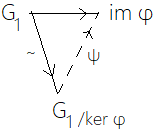
\includegraphics[width = 5cm]{constr.png}
\end{wrapfigure}

$G = (\mathbb{C} \backslash \{0\}, \times), H = S^{1} = {\tau: |z| = 1}, \; G_{\backslash H} \simeq (\mathbb{R}_{+}, \times), [z] \mapsto |z|.$

\textbf{Конструкция.} $\varphi: G_{1} \to G_{2},$ Im$\varphi \subset G_{2}$, где Im$\varphi$ --- подгруппа. Имеется отображение факторизации $\tau: G_{1} \to G_{1_{\backslash \ker \varphi}}, \; g \; \mapsto [g].$

\textbf{Лемма.} Существует гомоморфизм $\psi: G_{1_{\backslash \ker \varphi}} \to$ Im $\varphi,$ т.ч. $\varphi = \psi \cdot \iota.$ При этом $\psi$ является изоморфизмом. 
\section{Гомоморфизм групп} 

$\varphi: \; G_{1} \to G_{2},$ ker $\varphi = \{g \in G_{1}: \; \varphi(g) = e\},$ Im $\varphi = \{h \in G_{2}: \exists g \in G_{1}, \varphi(g) = h\}.$

ker $\varphi$ --- нормальная подгруппа, $G \backslash_{ker \varphi}$ --- факторгруппа. 

ker $\varphi = \varphi^{-1}(e).$ Как устроен прообраз неединичного элемента (слой над произвольным элементом)? 

Пусть $h \in G_{2}, \; g_{1}\widetilde{g} \in G_{1}$ т.ч. $\varphi(g) = \varphi(\widetilde{g}) = h.$ 

$\varphi(g) = \varphi(\widetilde{g}) \Leftrightarrow \varphi(g)\varphi(\widetilde{g})^{-1} = e \Leftrightarrow \varphi(g)\varphi(\widetilde{g}^{-1}) = e \Leftrightarrow \varphi(\widetilde{g}^{-1}) = e \Leftrightarrow gg^{-1} \in ker \varphi.$ 

$gg^{-1} \in$ ker $\varphi \; \Leftrightarrow g \in$ (ker $\varphi \widetilde{g}.$

\textbf{Лемма.} Все слои гомоморфизма $\varphi$ могут быть отождествлены с ker $\varphi$ (слой над $e \in G_{2}.$ 

\textbf{Доказательство.} Зафиксируем слой как прообраз $h \in G_{2}.$ Зафиксируем $g \in \varphi^{-1}(h).$ Тогда любой другой элемент в слое над $h$ имеет вид (ker $\varphi) \cdot g.$

\textbf{Следствие.} Если $|G_{1}|, \; |G_{2}| < \infty,$ то все слои содержат одинаковое количество элементов. 

\textbf{Предложение.} Любой гомоморфизм $phi: G_{1} \to G_{2}$ может быть разложен в композицию $G_{1} \to G_{1_{\backslash ker \varphi}} \to G_{2},$ где $p: G_{1} \to G_{1_{\backslash_{ker \varphi}}}, \; g \mapsto [g], \; i: G_{1 \backslash_{ker \varphi}} \to G_{2}, \; [g] \mapsto \varphi(g).$ 

\textbf{Доказательство.} $i$ корректно определно, т.к. если $[g_{1}] = [g_{2}],$ то $g_{1} = g_{2}h, \; h \in ker \varphi \Rightarrow \varphi(g_{1}) = \varphi(g_{2}h) = \varphi(g_{2}).$ Заметим, что $(ip)(g) = \varphi(g)$ по определению. Осталось проверить, что $i$ --- вложение, т.е. ker $i = e$ (или, равносильно, $i(x) = i(y) \Rightarrow x = y).$ Действительно, $i([g]) = e \Leftrightarrow \varphi(g) = e \Rightarrow e \in ker \varphi$ --- один класс в фактор-группе. 

Причем этот класс является единственным элементом в $G_{1 \backslash ker \varphi}.$ 

\textbf{Замечание.} Пусть $|G_{1}|, |G_{2}| < \infty.$ тогда $|im(\varphi)| = |G_{1}|_{\backslash_{|ker \varphi}|}.$

Группа преобразований --- действия групп на множествах. 

\textbf{Определение.} $X$ --- множество, Aut(X) --- группа всех взаимно-однозначных отображений $X \to X$ с операцией композиции. 

\textbf{Замечание.} Если $X$ конечно, то $Aut(X) \simeq S_{n},$ где $n = |x|.$ 

\textbf{Пример.} $X = \mathbb{N}, Aut(\mathbb{N}) = \{f: \mathbb{N} \to \mathbb{N} - \text{взаимно-однозначные отображения}\}.$ 

\textbf{Определения.} Любая подгруппа группы Aut(X) называется группой преобразований. 

\textbf{Замечание.} Абстрактная группа называется группой преобразований, если ее можно вложить в $Aut(X).$ 

\textbf{Пример.} Группа диэдра --- линейные преобразования $\mathbb{R}^{2},$ которые сохраняют правильный многоугольник. В качестве $X$ можно взять сам многоугольник (или множество его вершин). 

\textbf{Пример.} Группа преобразований куба.  

Бывают собственные и несобственные преобразования. 

Пусть $SO_{\text{куб}}$ --- собственные преобразования, которые сохраняют куб.

$x \mapsto -x$ --- несобственное. 

Пусть $X$ --- множество, состоящее из четырех диагоналей куба. Если $\varphi$ --- преобразование куба, то $\varphi$ индуцирует элемент $Aut(X).$ 

\textbf{Утверждение.} Мы получаем отображение из группы преобразований куба в Aut(X) = $S_{4}.$ При это любой элемент $S_{4}$ лежит в образе этого отображения. При этом отображение $x \to -x$ (центральная симметрия) индуцирует тождественное преобразование $X.$ 

Пусть $G \in Aut(X)$ --- группа преобразований. 

\textbf{Пример.} Пусть $\sigma \in S_{n}$ --- перестановка. Скажем, что $1 \leq i < j \leq n$ образуют инверсию (беспорядок), если $\sigma(i) > \sigma(j).$ Например, $\sigma = \begin{pmatrix}
1 & 2 & 3 \\
3 & 2 & 1
\end{pmatrix}; 13, 12, 23$ --- инверсии. Определим значение $\sigma$ на (-1). $\sigma$ называется четным, если ее знак 1, иначе нечетным. 

$\bullet$ [не расшифровала доску];

$\bullet$ преобразование $\delta \to \{\pm 1\}, \delta \mapsto sgn(\delta)$ --- гомоморфизм групп;

$\bullet$ четность перестановки совпадают с четностью количества транспозиций в различных перестановках на транспозиции;

$\bullet$ четные перестановки образуют группу, которая называется \textbf{знакопеременная группа} и обозначается $A_{n}.$ $|A_{n}| = \dfrac{n!}{2},$ т.к. $S_{n} = A_{n} \bigsqcup (12) A_{n}.$ 

В частности, $A_{n}$ --- группа преобразований $X = {1, 2, ..., n}.$ 

\subsection{Орбита, стабилизатор} 

\textbf{Определение.} \textbf{Орбита} $x \in X$ под действием $g$ --- множество $\{g.x\} \; g \in G.$ Обозначается $Gx.$ 

\textbf{Пример.} $G = Aut X, \; x \in X, Gx = X, \; G = id,$ то $Gx = \{x\}.$

\textbf{Замечание.} Разные орбиты не пересекаются. 

\textbf{Доказательство.} Пусть $x, y \in X, \; y \in Gx.$ Тогда $\exists g \in G: \; y = g.x \Rightarrow g^{-1}y \Rightarrow Gx = Gy.$

\textbf{Определение.} Стабилизатор точки $x \in X$ --- подмножество $Stab_{G}x \subset G,$ состоящее из $g: \; gx = g.$

\textbf{Замечание.} $Stab_{G} x$ --- подгруппа в $G,$ т.к. $(g_{1}g_{2}).x = g_{1}.(g_{2}.x).$ 

Как связаны стабилизаторы у двух разных точек в одной орбите? 

$Stab_{G}gx = \{g \in G: h.(g.x) = g.x\} = \{h \in G: (hg).x = g.x\} = \{g \in G: g^{-1}.(hg).x = g^{-1}(g.x)\} = \{h \in G: (g^{-1}hg).x = x\} = \{h \in G: g^{-1}hg \in Stab_{G}x\} = \{h \in G: \; h \in g Stab_{G}(x)g^{-1}\}.$ 

\textbf{Следствие.} Если $G$ --- конечная группа, то стабилизаторы всех точек в одной орбите равномощны. 

\textbf{Доказательство.} $a, b \in Stab_{G}x, \; a \neq b \Rightarrow gag^{-1} \neq gbg^{-1}.$ 

\textbf{Следствие.} $|G| = |Gx||Stab_{G}x|.$ 

\textbf{Доказательство.} $ev_{x}: G \to X.$ Тогда $|ev^{-1} (gx)| = |Stab_{G}gx| = |Stab_{G}x|.$ (т.к. $ker gx \subset G$ отображением $ev_{x}$ переходит в $gx \in G).$ $g \to g.x.$

\textbf{Следствие.} $|G|: |Gx|, |G|: |Stab_{G}x|.$  

$X$ --- множество, $G$ --- группа, Aut($X$) --- взаимно-однозначные отображения $X \to X.$ 

$G$ --- группа преобразований, если $G$ может быть реализована как подгруппа Aut(X). $\varphi: G \to$ Aut($X$), т.ч. $\varphi$ --- гомоморфизм, ker $\varphi = \{$id\}. 

\textbf{Определение.} $x \in X,$ орбита $Gx = \{y \in X: \; \exists g \in G \quad g.x = y\} \quad (gx = g.x = \varphi(g)x).$ Стабилизатор $x \in X$ --- подгруппа $Stab_{G}x = \{g \in G: \; gx = x\}.$ 

\textbf{Предложение.} Пусть $|G| < \infty. \; |Gx| = |G|_{/|Stab_{G}x}|. \; ev_{x}: G \to X, \; g \mapsto gx.$ 

\textbf{Определение.} $G$ --- группа, $X$ --- множество. $G$ действует на $X,$ если задан гомоморфизм групп $\varphi: G \to Aut(X).$ Другими словами, имеется отображение $G \times X \to X, \; (g_{1}x) \mapsto \varphi(g)x.$ 

\textbf{Замечание.} Отображение $\varphi$ может иметь ядро, т.е. могут существовать $g \in \varphi,$ т.ч. $\varphi(g) = id, \; g + e.$ 

\textbf{Определение.} Орбита: $\{y: \exists g \in G \quad gx = y\},$ стабилизатор $Stab_{G}x = \{g \in G: gx = x\}.$ 

\textbf{Замечание.} $\varphi: G \to Aut(X)$ --- действие, то Im$\varphi$ --- группа преобразований $X.$ 

\textbf{Замечание.} Любые две орбиты либо совпадают, либо не пересекаются. 

\textbf{Теорема.} Если конечная группа $G$ действует на $X,$ то $|Gx| = |G|_{/|Stab_{G}x|}.$ 

\textbf{Доказательство.} Рассмотрим $ev_{x}: G \to G_{x}, \; g \mapsto \varphi(g)x.$ Тогда легко проверить, что $\forall y \in G_{x}.$ $|ev_{x}^{-1}(y)| = |Stab_{G}x| \ni |G| = |G_{x}||Stab_{G}x|.$ 

\textbf{Замечание.} $G \overset{\varphi}{\rightarrow} Im \varphi, \; g \mapsto \varphi(g).$ У этого гомоморфизма есть ядро ker$\varphi.$ Пусть $a \in Im \varphi.$ Тогда $|\varphi^{-1}(a)| = |ker \varphi|,$ т.к. $\varphi(g_{1}) = \varphi(g_{2}) = a \Rightarrow \varphi(g_{1}g_{2}^{-1}) = id \Leftrightarrow g_{1}g_{2}^{-1} \in ker \varphi \Leftrightarrow g_{1} = \dfrac{ker\varphi}{g_{2}}.$ 

$Gx = (Im \varphi) x, \; |G| = |Im \varphi| |ker \varphi|, \quad |stab_{G} x| = |Stab_{Im\varphi}x| \cdot |ker \varphi|.$ 

\subsection{Транзитивность, точность, свободность} 

\textbf{Определение.} Действие $\varphi: G \to Aut(X)$ называется транзитивным, если $\forall x, y \in X \; \exists g \in G,$ т.ч. $gx = y.$ 

\textbf{Замечание.} У транзитивного действия ровно одна орбита. \textbf{Обозначение:} $X_{/G}$ --- множество орбит в $X$ при действии $G.$ 

\textbf{Определение.} Действие называется \textbf{свободным,} если из равенства $gx = x \quad (g \in G, \; x \in X) \Rightarrow g = e.$ Т.е. нет неединичных элементов, которые оставляют точку на месте. Иными словами, $Stab_{g}x = e \; \forall x \in X.$ 

\textbf{Определение.} Действие называется \textbf{точным,} если ker$\varphi$ = e. 

\textbf{Замечание.} Если действие \textbf{свободно,} то оно точно. Т.е. ни один элемент группы, кроме единичного, не переходит в тождественное преобразование. В обратную сторону неверно. 

\textbf{Пример. Левое действие группы на себя.} $X = G, \; L: G \to Aut(X), \; L(g)x = gx.$ 

\textit{Транзитивно.} Берем $x \in G, \; y \in G.$ Существует ли $g \in G: \; L(g)x = y \Leftrightarrow gx = y \Rightarrow g = yx^{-1}?$ Существует.

\textit{Точно.} Верно ли, что $L$ --- это вложение? ker L = $\{g \in G: L|g| = id\} = \{g \in G: \; gx \ x \; \forall x \in G\}.$ 

\textit{Свободно.} $gx = x \Leftrightarrow g = e.$ 

\textbf{Пример. Правое действие группы на себя.} $x = G, \; R: G \to Aut X, \; R(g)x = xg^{-1} \leftarrow$ гомоморфизм. Проверим. $R(g_{1}g_{2}) = R(g_{1})R(g_{2}) \Leftrightarrow \forall x: \; R(g_{1}g_{2})x = x(g_{1}g_{2})^{-1} = R(g_{1})(R(g_{2})x) = xg_{2}^{-1}g_{1}^{-1}.$ 

\textbf{Пример. Присоединенное действие.} Ad: $G \to Aut(X), \; X = G.$ $Ad(g)x = gxg^{-1}.$ 

\textit{Не транзитивно.} Если $G$ коммутативна, то Ad(g)x = x, т.е. Im Ad = \{id\}. Возьмем орбиту единичного элемента: $G_{e} = e,$ т.е. $e$ сдвинуть нельзя. 

\textit{Не точно.} Если $G$ коммутативно, то ker$\varphi$ = G. Вообще говоря, ker $\varphi = \{g \in G: \; gxg^{-1} = x \; \forall x\} = \{g \in G: gx = xg \; \forall x \in G\} = Z(G)$ --- центральная группа. 

\textit{Не свободно.}

\textbf{Пример.} $G = S_{n}.$ Хотим описать орбиты присоединенного действия. Пусть $\sigma$ --- перестановка, тогда $(Adg)\sigma = g \sigma g^{-1}.$ 

\textbf{Лемма.} $\sigma$ и $\tau$ лежат в одной орбите относительно присоединенного действия, если $\forall k = 1, 2, ..., n$ количество циклов длины $k$ в разложении $\sigma$ и $\tau$ на непересекающиеся циклы одинаковое. 

\textbf{Доказательство.} $(i_{1}i_{2}...i_{k})$ --- цикл, $g(i_{1}...i_{k})g^{-1} = (g(i_{1})...g(i_{k})).$ 

\textbf{Вопрос.} $\sigma \in S_{n},$ чему равна длина Ad-орбиты элемента $\sigma?$

\textbf{Предложение.} $|Stab_{S_{n}}\sigma| = m_{1}!m_{2}!...m_{n}!1^{m_{1}}2^{m_{2}}...n^{m_{n}} = \text{П}_{k = 1}^{n}k^{m_{k}}m_{k}!$ 

Пусть $\sigma$  разложена на непересекающиеся циклы и $m_{k}$ --- количество циклов длины $k$ в этом разложении. В частности, $m_{1} + 2m_{2} + ... + nm_{n} = n.$ 

\textbf{Доказательство.} Мы знаем, что $g(i_{1}i_{2}...i_{k})g^{-1} = (g(i_{1})...g(i_{k})).$ Поэтому если $g \sigma g^{-1} = \sigma,$ то для того, чтобы задать $g,$ нужно задать следующие данные: 

$\bullet$ для каждого цикла $(i_{1}...i_{k})$ нужно указать цикл длины $k$ в $\sigma,$ куда  начальный цикл перейдет; 

$\bullet$ для каждого цикла $(i_{1}...i_{k})$ нужно задать образ $f(i_{1})$ в соответствующем (выбранном) цикле длины $k.$ 

\textbf{Следствие.} Орбита перестановок $\sigma$ относительно присоединенного действия содержит $\dfrac{n!}{\text{П}^{n}_{k = 1} m_{k}!k^{m_{k}}}$ элементов. 

\textbf{Замечание.} Орбиты присоединенного действия называются классами сопряженных элементов. 

\subsection{Диаграммы Юнга}

\textbf{Диаграммы Юнга.} Пусть задан класс сопряженных элементов, т.е. $m_{1}, ..., m_{n}.$ 

\textbf{Пример.} $S_{27}, \; m_{1} = 2, m_{3} = 3, m_{5} = 2, m_{6} = 1.$ 

\textbf{Замечание.} Диаграмма Юнга из $n$ клеточек находятся во взаимно-однозначном соответствии с цикловыми типами в $S_{n} \Leftrightarrow$ классы сопряженных элементов. 
\end{document}

	